\part{CONTRATAÇÕES DE FORNECEDORES DE DESENVOLVIMENTO DE SOFTWARE}

\chapter[Contratações de Fornecedores de Desenvolvimento de Software]{Contratações de Fornecedores de Desenvolvimento de Software}

O descumprimento da legislação de licitações e contratos gera riscos para à contratação de tecnologia da informação e, portanto, devem ser conhecidos e usados como base de qualquer processo de contratação de fornecedores de desenvolvimento de software. Assim, neste Capítulo será apresentada uma visão sobre a importância da contratação de serviços de TI e a caracterização de contratação de tecnologia da informação pelas organizações públicas brasileiras segundo a legislação pertinente. Apresentando-se, de forma resumida os conceitos de contratação de serviços de TI presentes em normas, modelos, guias e processos de contratação de serviços de TI.

\section[Importância da Contração de Fornecedores de Desenvolvimento de Software]{Importância da Contração de Fornecedores de Desenvolvimento de Software}

Um dos principais, mais complexos e mais frequentemente utilizados atos administrativos é a contratação. Contratar é fazer contrato. Um contrato é um acordo ou convenção entre duas ou mais pessoas, para execução de alguma coisa, sob determinadas condições. O contrato é, portanto, o documento em que se registra esse acordo ou convenção \cite{MPOG:2011}.

Há vários anos, os órgãos da Administração Pública Federal (APF) têm adotado a prática da execução indireta de muitos serviços que dão suporte às suas áreas-fim, conhecida comumente como “terceirização de serviços”. O Decreto-Lei 200/1967 traz, no Art.10 § 7º, a diretriz para que a Administração Pública Federal se desobrigue da realização de tarefas executivas (execução de tarefas operacionais), recorrendo, sempre que possível, à execução indireta, desde que a iniciativa privada esteja suficientemente desenvolvida na área, bem como não haja comprometimento da segurança nacional (Art.10 §8º). De acordo com o Decreto-Lei 200/1967, Art.10, §7º, as razões para se partir para execução indireta são: possibilitar que a APF execute melhor as tarefas de planejamento, coordenação, supervisão e controle, tarefas que hoje podem ser traduzidas como gestão e governança; impedir o crescimento desmesurado da máquina administrativa, para que o Estado não alcance dimensão indevida em função da incorporação de tarefas de caráter operacional  \cite{TCU:2012}. 

Um levantamento do Tribunal de Contas da União (TCU) mostrou que o orçamento de gastos em TI da Administração Pública Federal de 2010 era de pelo menos 12,5 bilhões de reais, sendo grande parte desse valor destinado a contratações de serviços relacionados a software. No mesmo ano também era previsto um orçamento de cerca de 1,8 trilhão de reais da União, sendo que a maior parte seria gasto em TI. Com isso, os serviços de TI requerem bastante atenção e tem suma importância para administração pública brasileira, tanto no que diz respeito a contratações ou desenvolvimento de produtos de TI.

A definição e institucionalização de processos de contratação de serviços de TI, especialmente aqueles relacionados a software envolvem ações complexas, principalmente no que diz respeito à identificação dos requisitos necessários, a garantia da qualidade dos resultados esperados, os critérios de aceitação, a gestão de mudanças, as transferências de conhecimentos, a legislação pertinente, entre outros. E envolvem também questões de relacionamento entre clientes e fornecedores, o que implica em competências administrativas e jurídicas. Essas complexidades apresentam riscos para partes envolvidas e, como consequência, é comum a ocorrência de conflitos \cite{cruz2011}.

Assim, contratações envolvem riscos e incertezas oriundos de diversos fatores inerentes do objeto do contrato. Com isso, é preciso observar as características do objeto e do contexto em que ele será inserido, com especial atenção à conformidade legal em contratações de serviços de TI em organizações públicas, para que seja realizado o devido controle.


\section[Normas, Processos e Legislação Pertinentes à Contratação]{Normas, Processos e Legislação Pertinentes à Contratação}

\subsection[Lei nº 8.666/93]{Lei nº 8.666/93}

A Lei nº 8.666 \cite{Lei8666:1993} estabelece normas gerais sobre licitações e contratos administrativos. A licitação é tida como antecedente ao contrato administrativo. Pode ser considerado o procedimento no qual a Administração Pública escolhe a proposto mais vantajosa para contrato do seu interesse e ao mesmo tempo dá igual oportunidade aos que desejam fazer parte do contrato.

Uma licitação supõe concorrência entre ofertantes, portanto, os objetos propensos à licitação são aqueles que podem ser fornecidos por mais uma pessoa ou entidade. Os princípios da licitação de acordo com o Art. 3º são: igualdade, é impedido a existência de cláusulas no edital que favorecem um em detrimento de outros, mas não é considerado atentado ao principio da igualdade estabelecer requisitos mínimos de participação; legalidade, a licitação é um procedimento completamente vinculado à lei, todas suas fases não disciplinadas nesta lei, além disso, é possível a participação da população no controle do principio da legalidade na licitação, os Art.4º, Art.41, Art.101 e Art.113 prevê várias formas de participação popular; impessoalidade, a Administração deve considerar critérios claros e objetivos para escolha do licitante, todos devem ser tratados igualmente em termos de direito e obrigações; moralidade e probidade administrativa, é passível de punição qualquer comportamento que vá contra a moral, bons costumes, as regras de boa administração e aos princípios de justiça e equidade; publicidade, diz respeito tanto à divulgação da licitação para todos os interessados como também a que todos os atos praticados pela Administração durante todas as fases sejam abertos aos interessados, os Art. 3º, Art. 4º, Art.15, Art.16 e Art.43 deixam esse princípio claro; vinculação ao instrumento convocatório,  o edital deve estar vinculado à licitação e sua alteração só é permitida quando for falho ou inadequado ao interesse público, o Art. 41 deixa esse princípio claro; julgamento objetivo, previsto no Art. 3º, diz respeito a utilizar o critério indicado no ato convocatório para julgamento das propostas, seja ela técnica ou de preço; fiscalização da licitação, diz respeito a qualquer cidadão poder controlar a licitação contra irregularidades na aplicação da lei de licitação, como disposto nos Art.4º, Art.8º, Art.63 e Art.113; competitividade, a lei proíbe a existência de cláusulas que vá contra o caráter competitivo da licitação, com ressalva em casos de só haver um interessado ou um concorrente após a fase de classificação; e a padronização, que sempre que possível deve ser adotada a padronização como estabelecido no Art. 15; 

A Lei 8.666 prevê cinco modalidades de licitação no Art. 22: concorrência, tomada de preços, convite, concurso e leilão, elas estão relacionadas ao valor estimado do contrato. O pregão foi criado como modalidade de licitação pela medida provisória nº 2.026 e na lei nº 10.520. As modalidades sem finalidade específica entram no grupo formado pela concorrência, pela tomada de preços e pelo convite. O grupo das modalidades com finalidades específicas é formado pelo concurso e pelo leilão. Os quatro tipos de licitação presentes no Art.45 são: menor preço, melhor técnica, técnica e preço e maior lance ou oferta, elas estão relacionas com o julgamento.

As fases da licitação são: a interna, que é destinada a firmar a intenção da entidade licitante e a obter informações necessárias para a consolidação da licitação; e a externa, que é destinada a selecionar a melhor proposta. A fase interna é composta por determinar o objeto de licitação, as condições, a estimativa de despesas e a decisão pela modalidade mais adequada, além da verificação da existência de recursos e a obtenção da autorização de abertura do instrumento convocatório.

A fase externa é dividida de forma geral em: abertura; habilitação, classificação; e julgamento.  A abertura é o momento em que o instrumento convocatório, edital ou carta-convite é tornado conhecido publicamente. O edital é composto por preâmbulo, texto e fecho. Segundo Art. 40, no texto do edital devem estar: as condições relacionadas à apresentação das propostas e à participação dos licitantes; os critérios de julgamento das propostas; a descrição resumida do objeto da licitação; o prazo de execução; as garantias; os recursos admissíveis; os critérios de desempate;  o prazo e condições para assinatura do contrato; as sanções para o caso de inadimplência; as condições de pagamento; as condições de recebimento do objeto da licitação; e os critérios de reajustamento.

A habilitação é onde a comissão de licitação confirma os licitantes aptos a participarem da licitação de acordo com o edital. As condições para conseguir a habilitação são: habilitação jurídica; qualificação técnica; qualificação econômico-financeira; regularidade fiscal; não empregar menores de 18 anos em trabalho noturno, perigoso ou insalubre, ou menores de 16 anos, salvo a partir dos 14 anos na condição de aprendiz. 

A classificação é o ato o qual a comissão de licitação reúne as propostas apresentadas formalmente e de acordo com o edital ou carta-convite que são aptas para classificação e as que não estão conforme edital ou carta-convite são desclassificadas. O julgamento costuma ocorrer logo após a classificação das propostas. Para o julgamento é considerado apenas o foi permitido no instrumento convocatório e é feito de acordo com um dos quatro tipos de licitação, aquele que foi previsto no edital. 

A licitação do tipo menor preço é aquela que o fator de decisão é apenas o menor preço, as demais características como qualidade e produtividade não são consideradas. A licitação do tipo melhor técnica não considera só o preço, considera as melhores tecnologias, aquelas mais modernas ou que satisfaçam da melhor forma as necessidades da Administração licitante e que estejam dentro dos recursos financeiros disponíveis. A licitação do tipo técnica e preço é aquele em que é feita uma ponderação para técnica e preço a fim de considerar ambos. E a licitação do tipo maior lance ou oferta é aquele em que é escolhida a proposta que faz a maior oferta, este tipo é especialmente usado em vendas de bens ou permissões de uso de bens ou serviços públicos.

Após o julgamento, é realizado o processo de homologação e adjudicação. Na homologação, uma autoridade competente, indicado por lei, promove o controle de todo o processo licitatório no que diz respeito à legalidade. E na adjudicação é  atribuído ao vencedor da licitação o objeto da licitação pela mesma autoridade competente. Outros detalhes da Lei 8.666 não foram considerados pertinentes para o escopo desse trabalho.


\subsection[Instrução Normativa nº 04]{Instrução Normativa nº 04}

A Instrução Normativa nº 04 \cite{IN04:2010} disciplina sobre o processo de Contratação de Soluções de Tecnologia da Informação pelos órgãos integrantes do Sistema de Administração dos Recursos de Informação e Informática do Poder  Executivo Federal e é a consolidação de um conjunto de boas práticas para Contratação de Solução de TI pela Administração Pública Federal. Este conjunto de boas práticas é chamado de Modelo de Contratações de Soluções de TI (MCTI). Esta Instrução Normativa está dividida em três capítulos. O primeiro capítulo diz respeito às Disposições Gerais. O segundo capítulo diz respeito ao Processo de Contratação. E o terceiro capítulo diz respeito às Disposições Finais.

De forma geral no capítulo das Disposições Gerais é mencionado os atores, os artefatos e o que é vedado no processo de contratações.  Os atores considerados no processo de contratação de acordo com Art. 2º são: 

\begin{itemize}
\item Área requisitante da solução, que é a entidade ou órgão que demanda a contratação de uma Solução de Tecnologia da Informação; 
\item Área de tecnologia da informação, que é a unidade setorial do SISP responsável por gerir a Tecnologia da Informação do órgão ou entidade;
\item Equipe de planejamento da contratação, constituída pelo integrante técnico (servidor da área de TI), integrante administrativo (servidor da área administrativa) e integrante requisitante (servidor da área requisitante);
\item Gestor do contrato, que é o servidor com atribuições gerenciais, técnicas e operacionais responsável pela gestão do contrato; 
\item Fiscal técnico do contrato (servidor da área de TI); 
\item Fiscal administrativo do contrato (servidor da área administrativa); 
\item Fiscal requisitante do contrato (servidor da área requisitante);
\item Contratada, entidade provedora da Solução de Tecnologia da Informação;
\item Preposto, que é o funcionário representante da contratada, responsável por acompanhar a execução do contrato e atuar como interlocutor principal junto à contratante.
\end{itemize}

Os artefatos que podem ser produzidos e fornecidos para contratada ou recebidos pelo contratante são: a solução de tecnologia da informação; os requisitos; o documento de oficialização da demanda; a análise de viabilidade da contratação; o plano de sustentação; a estratégia da contratação; a análise de riscos; o plano de inserção; a ordem de serviço ou de fornecimento de bens; o termo de recebimento provisório; o termo de recebimento definitivo; os critérios de aceitação; a gestão e o plano diretor de tecnologia da informação.

Dentro das Disposições Gerais é ressaltado no Art.5º que não poderão ser objetos de contratação mais de uma solução de TI em um único contrato e a gestão de processos de TI.  No Art. 6º é dito que a contratada que provê a solução de TI não poderá ser a mesma que realiza medições, avaliação ou fiscalização. E é vedado, segundo Art. 7º prever a remuneração dos funcionários da contratada já no edital, reembolsar despesas que são de exclusiva responsabilidade da contratada, exigir qualquer tipo de capacitação ou certificação no edital, demandar aos funcionários da contratada tarefas fora do escopo do objetivo da contratação  e indicar pessoas para compor o quadro funcional da contratada. 

Neste capítulo está ainda a Estratégia Geral de Tecnologia da Informação (EGTI) que contém orientações gerais para as áreas de TI e dos órgãos e entidades da Administração Pública Federação e a formulação de um Plano Diretor de Tecnologia da Informação (PDTI) por parte de cada entidade integrante do Sistema de Administração dos Recursos de Informação e Informática (SISP) do Poder Executivo Federal, de forma geral neste documento são apresentados a avaliação e o diagnóstico dos recursos de TI, as necessidades da entidade e o planejamento de investimentos e recursos.

O Capítulo dois sobre o Processo de Contratação, que é de fato o MCTI, divide as contratações de soluções de TI em três fases: Planejamento da Contratação (PCTI); Seleção do Fornecedor (SFTI) e Gerenciamento do Contrato (GCTI).

\begin{figure}[h]
		\centering
		\label{fig05}
			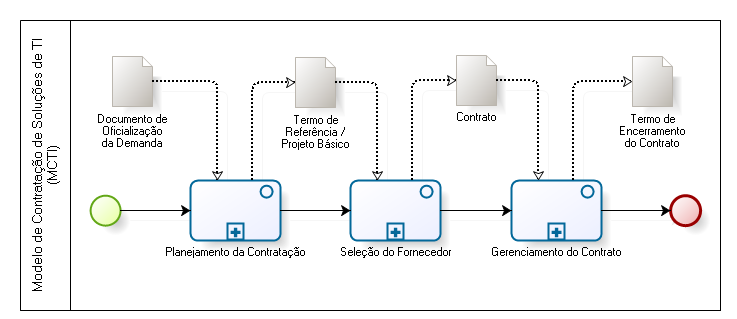
\includegraphics[scale=0.8]{figuras/MCTI.png}
		\caption{Modelo de Contratações de Soluções de TI   \cite{mcti}}
\end{figure}


Cada fase é constituída de processos/etapas, atividades, artefatos e atores conforme mostrado na tabela 1.
  
\begin{table}[htb]
\center
\footnotesize
\begin{tabular}{|p{1.4cm}|p{1cm}|p{3cm}|p{3cm}|p{3cm}|}
  \hline
   \textbf{Fases} & \textbf{Etapas}  & \textbf{Atividades}  & \textbf{Artefatos} & \textbf{Atores}  \\
    \hline
    PCTI & 5 & 41 & 8 & 7\\
   \hline    
    SFTI & 3 & 7 & 1 & 4\\
    \hline
    GCTI & 5 & 19 & 4 & 5\\
   \hline
\end{tabular}
\caption{Fases do MCTI}
\end{table}


No Planejamento da Contratação é necessário no mínimo ter no documento quais são as necessidades corporativas da instituição e seus objetivos estratégicos, motivação, resultados esperados, fonte de recursos e a indicação do integrante requisitante que fará parte da equipe de planejamento.  Após o recebimento desse documento a área de TI indicará, então, o integrante técnico que também fará parte da equipe de planejamento. E finalmente, o documento será encaminhado para a área administrativa, a qual indicará o integrante administrativo que fará parte da equipe de planejamento e dará prosseguimento para a contratação. Assim, a equipe de planejamento da contratação estará completa para acompanhar e apoiar todas as atividades presentes nas fases de planejamento da contratação e seleção do fornecedor.

A fase de Planejamento da Contratação é obrigatória independentemente do tipo de contratação, deve ser elaborada em harmonia com o PDTI e contém cinco etapas: análise de viabilidade; plano de sustentação; estratégia da contratação; análise de riscos; e termo de referência ou projeto básico. A análise de viabilidade da contratação compreende a definição e especificação de requisitos levando em conta que compete ao integrante técnico especificar os requisitos tecnológicos e ao integrante requisitante os demais requisitos, a identificação de possíveis soluções, análise e comparação de custos totais dessas soluções, a escolha da solução de TI e a justificativa da solução escolhida e avaliação das necessidades de adequação para viabilização da execução contratual. 

O plano de sustentação, que deve conter quais os recursos materiais e humanos que serão necessários, atividades de transição contratual e encerramento do contrato, assim como a continuidade do fornecimento da solução de TI em caso de interrupção contratual e a estratégia de independência do contratante com relação à contratada. 

A estratégia da contratação será elaborada a partir das duas etapas anteriores e conterá a indicação da solução de TI a ser contratada, definição das responsabilidades da contratada além das responsabilidades estabelecidas no contrato, a indicação dos termos contratuais observando os elementos contidos na Lei nº 8.666, de 1993, a elaboração do orçamento detalhado, da estimativa do impacto econômico-financeiro no orçamento do órgão requisitante, a elaboração dos termos de compromisso e sigilo, a definição dos critérios técnico de julgamento das propostas para a fase de seleção de fornecedor. 

A análise de riscos deverá conterá identificação dos principais riscos que podem comprometer o sucesso dos processos de contratação e de gestão contratual ou que possam fazer com que a solução de TI não atenda às necessidades esperadas, a mensuração das probabilidades de ocorrência e dos dados potenciais relacionados a cada risco, a definição das ações de contingência em caso de ocorrência dos ricos e a definição dos responsáveis pelas ações de prevenção e de contingência dos riscos.

E o termo de referência ou projeto básico que deverá conter no mínimo a definição do objetivo, a fundamentação da contratação, a descrição da solução de TI, os requisitos da solução, o modelo de prestação de serviços ou de fornecimentos de bens, os elementos para gestão do contrato, a estimativa de preços, a adequação orçamentária, as definições dos critérios de sanções e os critérios de seleção do fornecedor. 

Na fase de Seleção de Fornecedor deverão ser observadas as normas pertinentes e tem como recomendação a utilização da modalidade de Pregão na forma eletrônica devido à padronização existente no mercado de TI.  A área de licitações conduzirá esta fase a cabe a área de TI analisar as sugestões feitas, apoiar tecnicamente o pregoeiro na reposta à questionamentos e na análise e julgamento das propostas e dos recursos apresentados pelos licitantes. No encerramento desta fase, além do contrato, terá a nomeação do gestor do contrato, do fiscal técnico do contrato, do fiscal requisitante do contrato e do fiscal administrativo do contrato.


A fase de Gerenciamento do Contrato visa acompanhar e garantir a adequado prestação do serviço e o fornecimento de bens que compõem a solução de TI e compreende as seguintes etapas: início do contrato; encaminhamento formal de ordem de serviço ou fornecimento de bens; monitoramento da execução; e transição contratual e/ou encerramento do contrato. O início do contrato abrange a elaboração do plano de inserção da contratada, que contempla o repasse de conhecimento e a disponibilização de infraestrutura, e uma reunião inicial que tem como objetivo a entrega do termo de compromisso e do termo de ciência e de sigilo assim como possíveis esclarecimentos. 

\begin{figure}[h]
		\centering
		\label{fig05}
			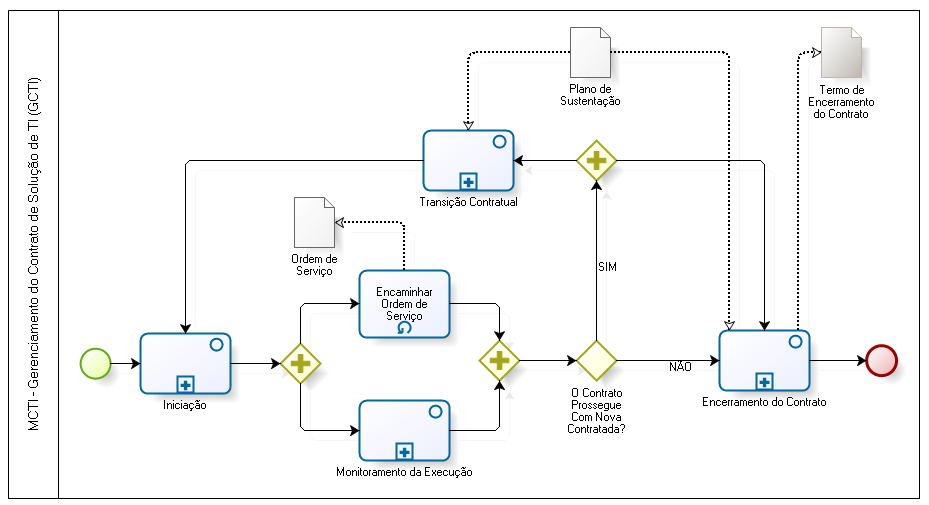
\includegraphics[scale=0.6]{figuras/GCTI.png}
		\caption{Gerenciamento de Contratações de Soluções de TI   \cite{mcti}}
\end{figure}

O encaminhamento formal de ordem de serviço ou fornecimento de bens pelo gestor do contrato para o preposto da contratada deve conter a definição e especificação dos serviços prestados ou bens fornecidos, o volume dos serviços ou quantidade de bens segundo métricas, o cronograma e a identificação dos responsáveis pela solicitação da solução de TI. 

O monitoramento da execução consiste da confecção e assinatura do termo de recebimento provisório, na avaliação da qualidade do serviço, na identificação de não conformidade, na verificação de aderência aos termos contratuais, na verificação da manutenção das condições classificatórias, no encaminhamento das demandas de correção à contratada, no encaminhamento de indicações de sanções, na confecção e assinatura do termo de recebimento definitivo, na autorização para emissão de nota fiscal, na verificação das regularidades fiscais, trabalhistas e previdenciárias, na verificação de manutenção de necessidade, economicidade e oportunidade da contratação, no encaminhamento de pedidos de modificação contratual e na manutenção do histórico de gerenciamento de contrato. 

E por fim a etapa de transição contratual ou encerramento do contrato que deverá observar o Plano de Sustentação. Vale ressaltar que para cada contrato, deverá haver pelo menos uma Ordem de Serviço ou de Fornecimento de Bens e pode haver quantas forem necessárias para execução do objeto contratado.


\subsection[Processo de Contratação de Serviços Tecnologia da Informação]{Processo de Contratação de Servços Tecnologia da Informação}

O propósito do Processo de Contratação de Serviços de Tecnologia da Informação para Organizações Públicas (PCSTI), de 2011, é obter \textit{software} e serviços de TI que satisfaçam às necessidades de negócio da organização contratante, de forma alinhada à sua estratégia e à legislação brasileira, considerando a necessidade de cumprir os princípios de eficácia, eficiência, efetividade, economicidade, legalidade e legitimidade dos projetos de TI. Este processo pode ser adotado para contratação de qualquer tipo de serviço de TI no setor público.

A estrutura do PCSTI é composta por quatro fases, dezoito atividades e 90 tarefas. As fases são: planejamento de TI; planejamento da contratação; seleção do fornecedor; e gestão do contrato.  A fase de Planejamento de TI é a fase em que são escolhidas as ações de TI de acordo com a estratégia de cada organização para produzirem os benefícios de negócio que foram priorizados. Esta fase é composta de duas atividades: estabelecer diretrizes para uso organizacional de TI e estabelecer o plano de contratações do PDTI.

A fase de Planejamento da Contratação é aquela em que todos os elementos da contratação são definidos de forma a garantir os príncipios de economicidade, efetividade, eficiência e eficácia.  As atividades relacionadas a esta fase são: analisar a viabilidade, elaborar o plano de sustentação, elaborar a estratégia de contratação, analisar e tratar riscos e concluir o planejamento da contratação.

A fase de Seleção do Fornecedor é aquela em que o modelo de prestação de serviços, a análise do mercado, o modelo de gestão do contrato e o modelo de seleção do fornecedor são utilizados para selecionar o fornecedor mais adequado às necessidades da Administração. As atividades desta fase são: formalizar e aprovar o termo de referência, selecionar fornecedor e formalizar contrato.

E a fase de Gestão do Contrato é aquele em que há o controle da execução do contrato de forma a alcançar os benefícios de negócio que foram previstos inicialmente.  As atividades relacionadas a esta fase são: iniciar o contrato, encaminhar demandas, realizar o monitoramento técnico, executar a atestação técnica, realizar o monitoramento administrativo, tratar as demandas por alterações contratuação e realizar o encerramento contratual e a transição.



